\documentclass[aspectratio=169]{beamer}

\mode<presentation>
{
  \usetheme{Spil}
  \setbeamercovered{invisible}
}

\usepackage[english]{babel}
\usepackage[latin1]{inputenc}

\usepackage{times}
\usepackage[T1]{fontenc}

% Anchoring images
%\usepackage[absolute, overlay]{textpos}

\title[]{\alert{Spilgames Storage Platform}}

\author[]{Enrique Paz}
%\author{\texorpdfstring{Author\newline\url{email@email.com}}{Author}}

\institute[] % (optional, but mostly needed)
{Senior Backend Developer}

\date[]{21/03/2013}

\AtBeginSection[]{
    \begin{frame}
        \begin{center}
            \huge{\insertsectionhead}
        \end{center}
    \end{frame}
}

\begin{document}

\begin{frame}
    \titlepage
\end{frame}

\section{Introduction}
\subsection{Spilgames \& Me}

\begin{frame}{About Me}
    \begin{columns}
        \begin{column}[c]{0.05\textwidth}
        \end{column}
        \begin{column}[c]{0.2\textwidth}
            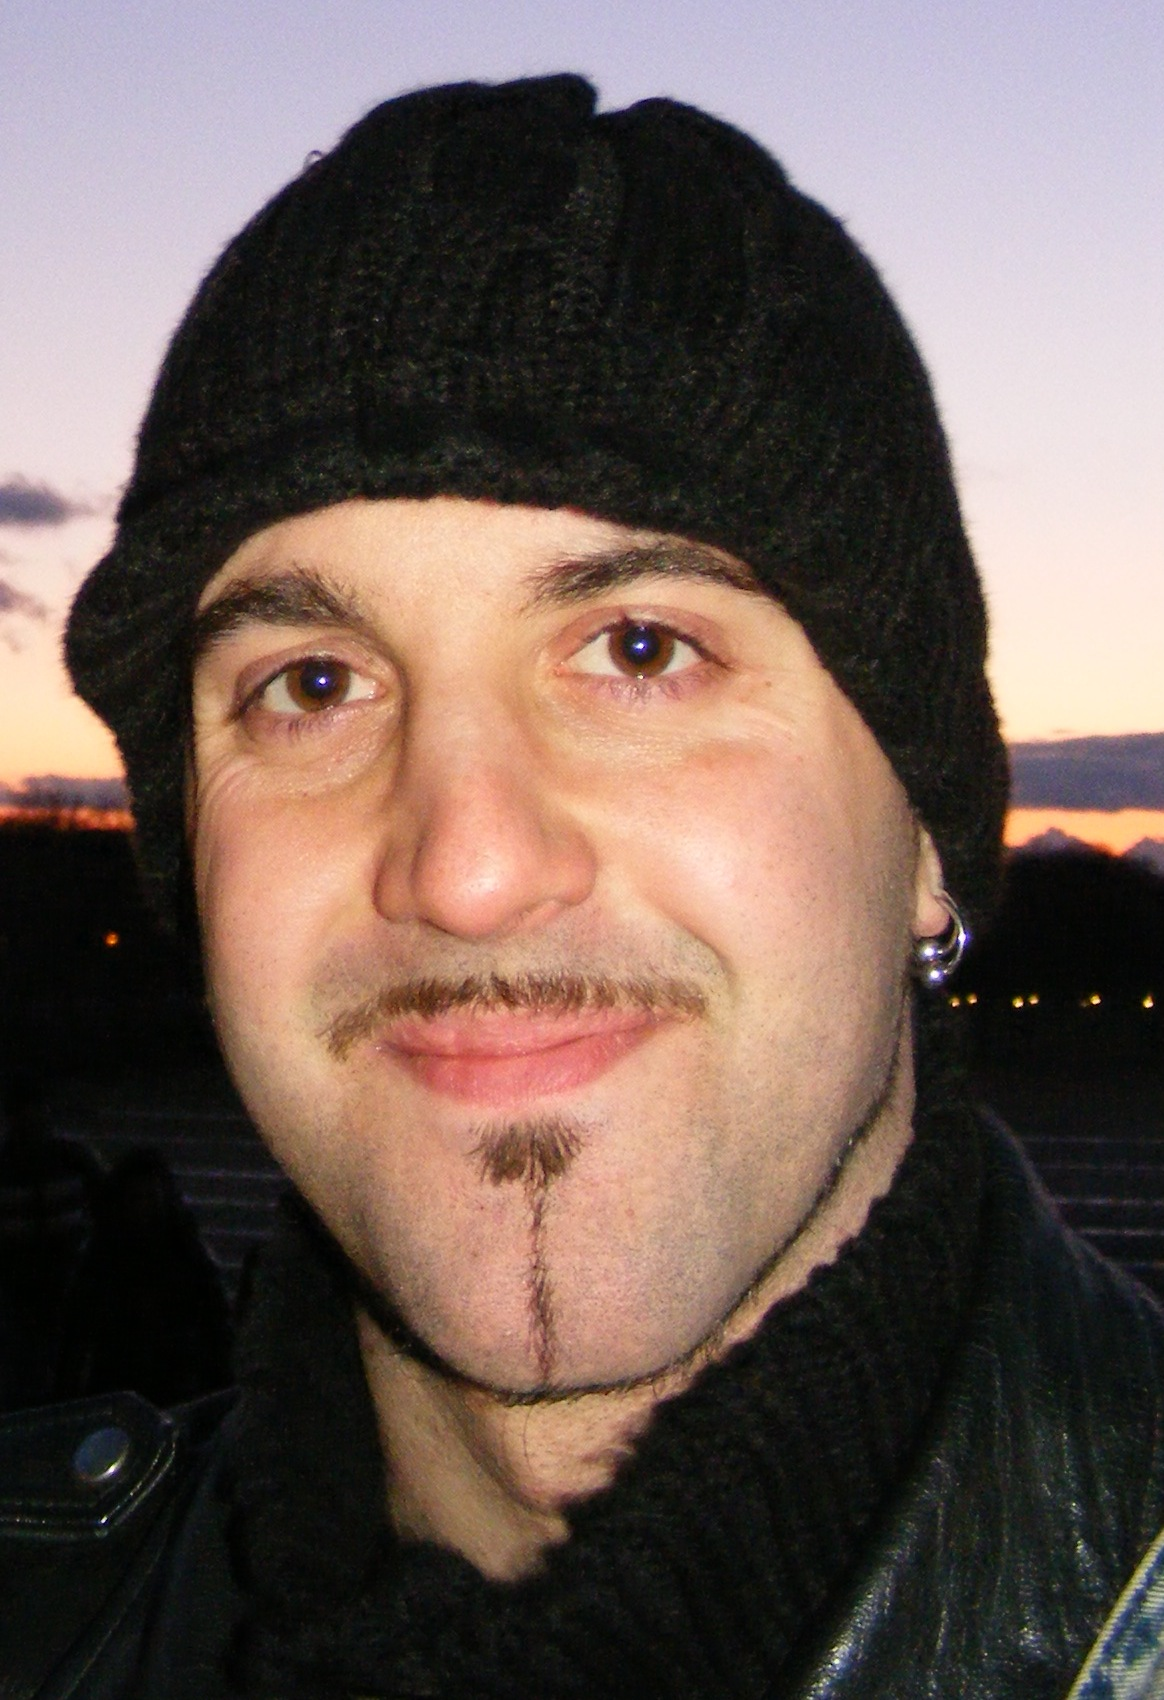
\includegraphics[width=\textwidth]{images/me.png}
        \end{column}
        \begin{column}[c]{0.05\textwidth}
        \end{column}
        \begin{column}[c]{0.7\textwidth}
            \begin{itemize}
                \item Passionate Erlang Developer
                \item Testing Enthusiast
                \item Development Process Caretaker
                % \item Triumph Rider
                % XXX Picture with the bike
            \end{itemize}
        \end{column}
    \end{columns}
\end{frame}

\begin{frame}{Spilgames}
    \begin{itemize}
       \item Gaming Platform
       \item Serving data to 190+ countries world-wide
       \item 180+ million unique users per month
       \item Multiple Platforms: Desktop, Mobile Native \& Web
       \item 300+ employees
       \item Offices in The Netherlands \& China
       \item Revenue: Advertising \& EUM
    \end{itemize}
\end{frame}

\begin{frame}{Gaming Portals}
    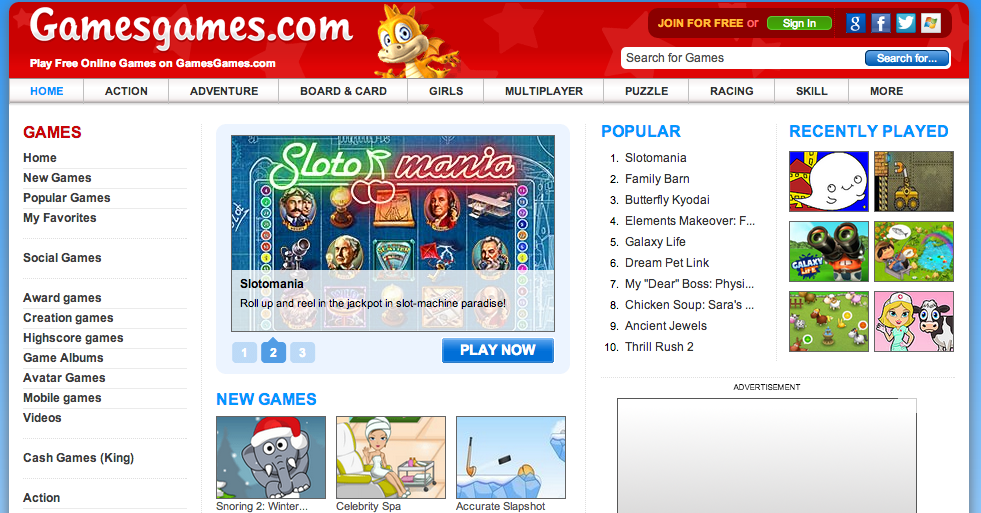
\includegraphics[width=\textwidth]{images/gamesgames.png}
\end{frame}

\begin{frame}{Gaming Portals}
    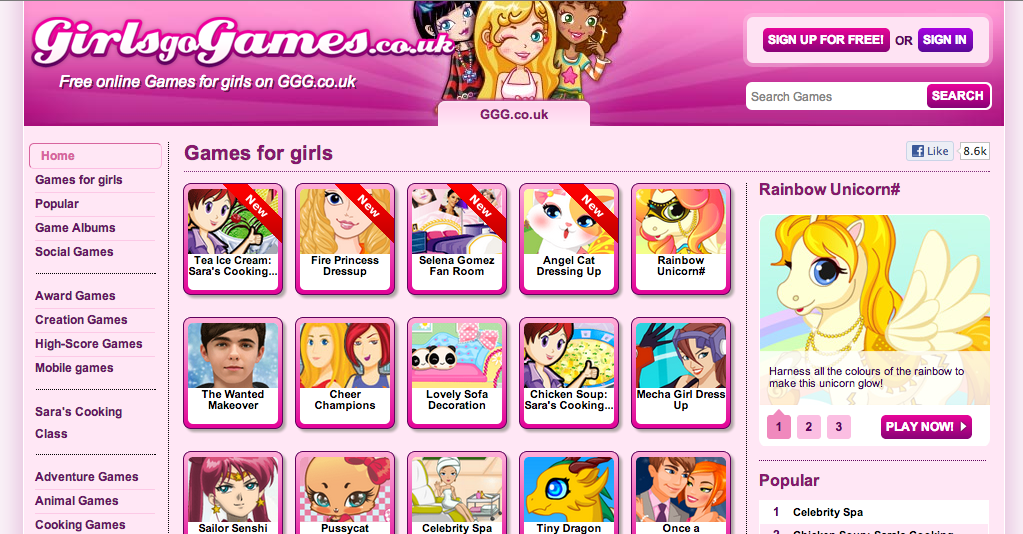
\includegraphics[width=\textwidth]{images/ggg.png}
\end{frame}

\begin{frame}{Games}
    \begin{columns}
        \begin{column}[c]{0.5\textwidth}
            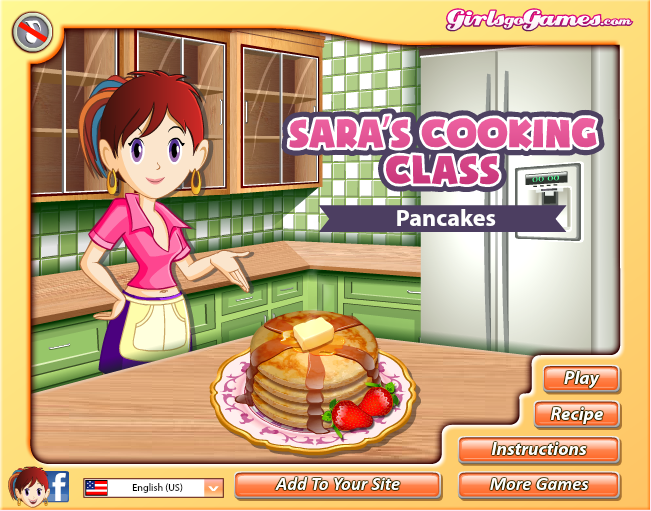
\includegraphics[height=0.6\textheight]{images/sarah.png}
        \end{column}
        \begin{column}[c]{0.5\textwidth}
            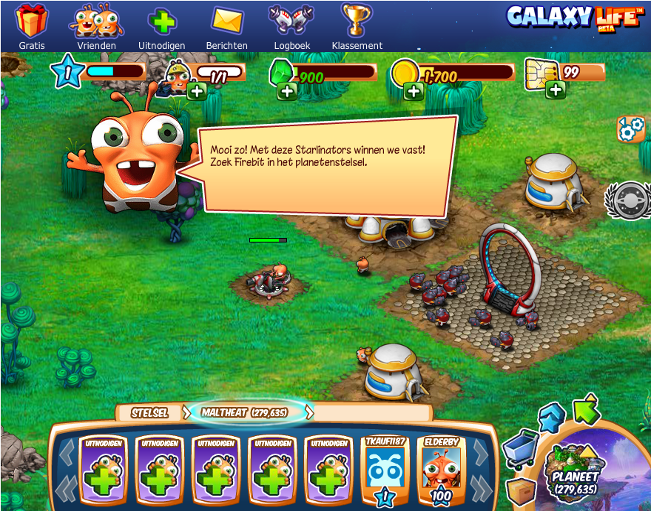
\includegraphics[height=0.6\textheight]{images/galaxylife.png}
        \end{column}
    \end{columns}
\end{frame}

\section{Another Storage}

{
\usebackgroundtemplate{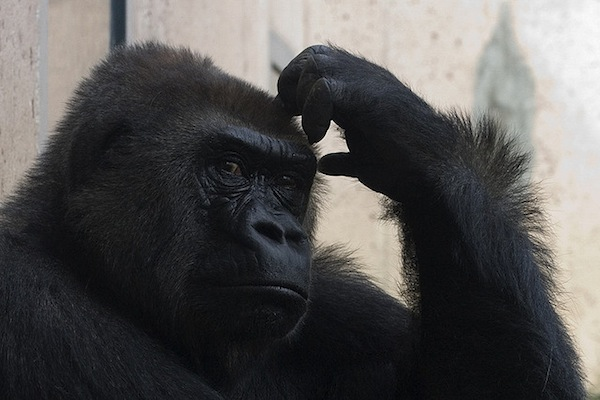
\includegraphics[width=\paperwidth]{images/anotherstorage.png}}
\begin{frame}{Another Storage}
\end{frame}
}

\subsection{Motivation}

\begin{frame}{LAMP Stack \& MySql}
    \begin{columns}
        \begin{column}[c]{0.6\textwidth}
            \begin{itemize}
                \item Not all developers are DB experts
                \item Difficult to shard the databases
                \item Storage model all over the place
                \item Security
                \item Performance
                \item Caching
                \item \dots
            \end{itemize}
        \end{column}
        \begin{column}[c]{0.4\textwidth}
            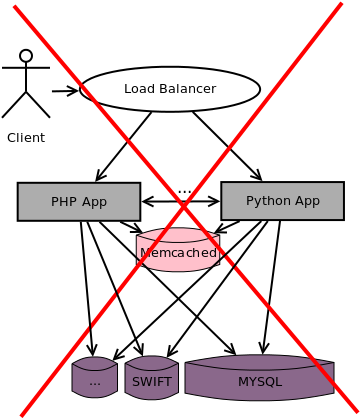
\includegraphics[width=0.9\textwidth]{images/oldstorageusage.png}
        \end{column}
    \end{columns}
\end{frame}

\begin{frame}{Our Ambition}
    \begin{columns}
        \begin{column}[c]{0.6\textwidth}
            \begin{itemize}
                \item Transparent sharding layer
                \item Sharding based on data ownership
                \item High Availability
                \item Centralized caching layer
                \item Storage engine agnostic
                \item Strict data model defined in one place
                \item Changing storage shouldn't affect business
                \item Ability to scale geographically
            \end{itemize}
        \end{column}
        \begin{column}[c]{0.4\textwidth}
            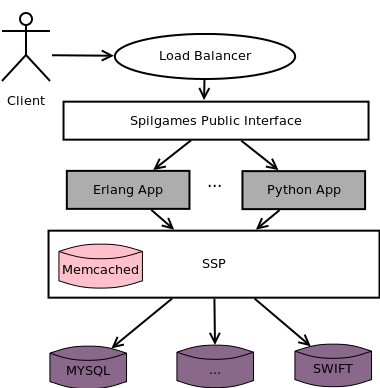
\includegraphics[width=0.9\textwidth]{images/newstorageusage.png}
        \end{column}
    \end{columns}
\end{frame}

\section{System Properties}

\subsection{Overview}

\begin{frame}{Mindset}
    \begin{itemize}
        \item Always available
        \item No global locks
        \item Inconsistencies are the norm
            \begin{itemize}
                \item Hardware breaks down (power failures)
                \item Version mismatches (upgrading system not atomic)
                \item State mismatches (adding new machines)
            \end{itemize}
    \end{itemize}
\end{frame}

\begin{frame}{A Key-Value Store With Schema}
    \begin{itemize}
        \item \textbf{Buckets}
            \begin{itemize}
                \item Largely generated OTP applications
                \item Offer a CRUD-like interface (with filters)
            \end{itemize}
        \item \textbf{GID}s identify the data owner
            \begin{itemize}
                \item user
                \item game
            \end{itemize}
        \item Buckets can use different storage engines:
            \begin{itemize}
                \item Several MySql tables in different databases
                \item Just a binary storage (SWIFT)
                \item \dots
            \end{itemize}
        \item Data for a bucket/GID is cached
        \item Requests can be atomic per bucket/GID
    \end{itemize}
\end{frame}

\begin{frame}{Optimistic Operations}
    \begin{itemize}
        \item Speed > Consistency
        \item Losing some updates in case of crash is affordable
        \item Destructive operations act first on cache and eventually on disk
        \item No warranties of eventual consistency upon crashes
            \begin{itemize}
                \item i.e. Activity feeds
                \item i.e. Popular Games List
            \end{itemize}
    \end{itemize}
\end{frame}

\begin{frame}{Pessimistic Operations}
    \begin{itemize}
        \item Consistency is key and confirmation is required
        \item Dealing with critical data
        \item Destructive operations act on disk and, upon success, on cache
            \begin{itemize}
                \item i.e. Payments
                \item i.e. Personal Information
            \end{itemize}
    \end{itemize}
\end{frame}

\subsection{Internals}
{
\usebackgroundtemplate{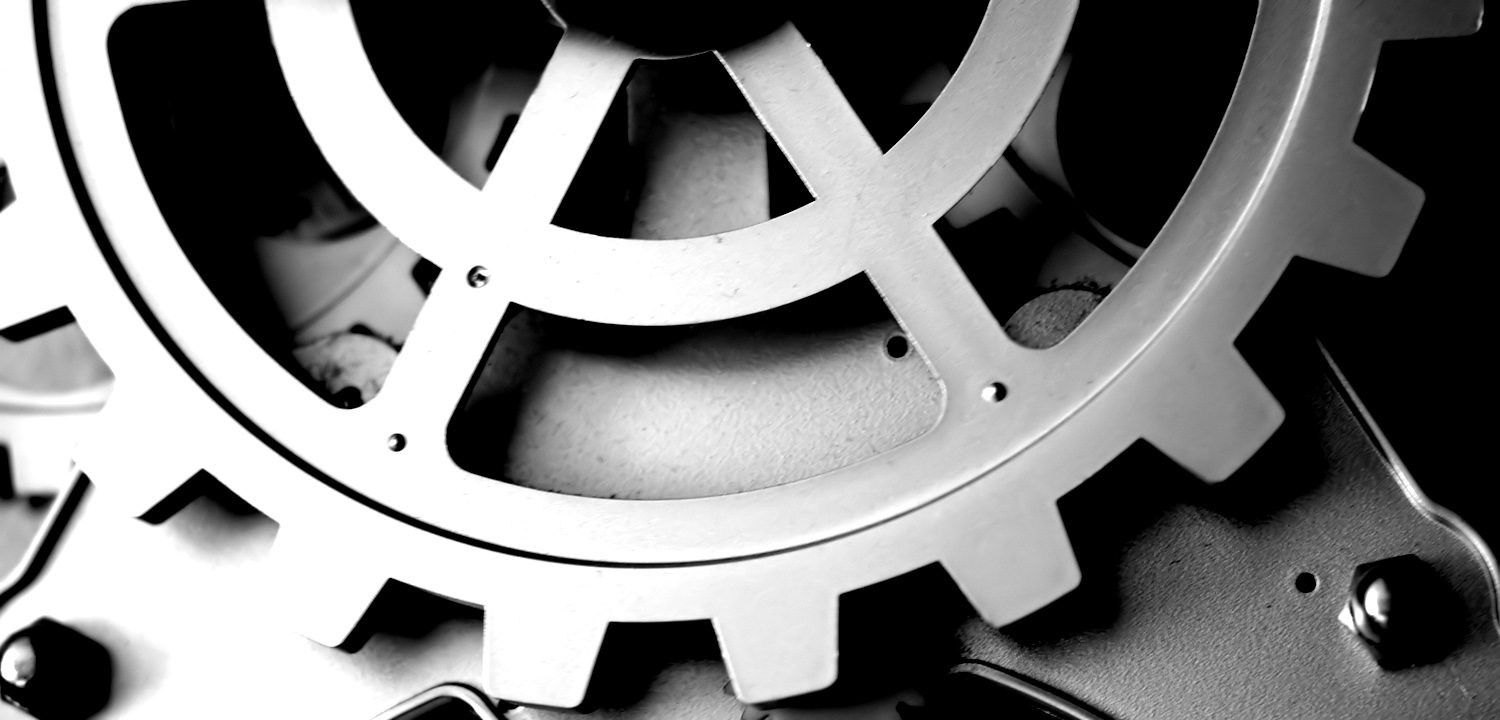
\includegraphics[height=\paperheight]{images/howitworks.png}}
\begin{frame}{How does it work?}
\end{frame}
}

\begin{frame}{System Components}
    \begin{columns}
        \begin{column}[c]{0.6\textwidth}
            \begin{itemize}
                \item \textbf{lookup} application \& lookup \textbf{hashing ring}
                \item \textbf{Buckets} register their \textbf{PF}s in the local lookup application
                \item The hashing ring is a distributed mnesia table:
                    \begin{itemize}
                        \item ram\_copies
                        \item dirty reads
                        \item transactional writes
                    \end{itemize}
            \end{itemize}
        \end{column}
        \begin{column}[c]{0.4\textwidth}
            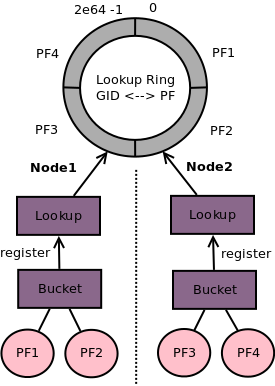
\includegraphics[height=0.7\textheight]{images/components.png}
        \end{column}
    \end{columns}
\end{frame}

\begin{frame}{Tracing Pessimistic Operations}
    \begin{columns}
        \begin{column}[c]{0.6\textwidth}
            \begin{enumerate}
                \item Random SSP node receives request for bucket/GID
                \item Node uses local lookup to find the PF
                \item PF receives the original request
                \item PF builds the job to be executed
                \item If none, PF creates a pipeline for GID
                \item PF queues the operation in pipeline for GID
            \end{enumerate}
        \end{column}
        \begin{column}[c]{0.4\textwidth}
            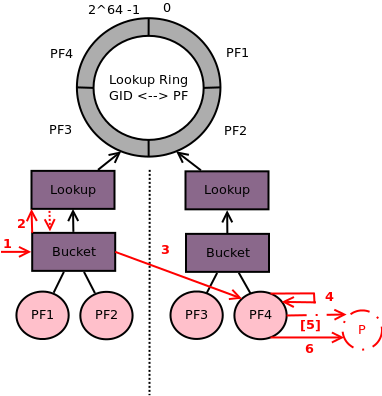
\includegraphics[width=\textwidth]{images/tracingpessimistic.png}
        \end{column}
    \end{columns}
\end{frame}

\begin{frame}{Wait a minute\dots}
    \begin{columns}
        \begin{column}[c]{0.05\textwidth}
        \end{column}
        \begin{column}[c]{0.3\textwidth}
            
\includegraphics[width=0.8\textwidth]{images/slow.png}
        \end{column}
        \begin{column}[c]{0.65\textwidth}
            \begin{itemize}
                \item ``Why do we need pipelines?''
                \item ``Sequential == Bottleneck !!!''
                \item ``Don't you guys know Erlang is about \textbf{parallelizing} work?''
            \end{itemize}
        \end{column}
    \end{columns}
\end{frame}

\begin{frame}{About Pipelines}
    \begin{itemize}
        \item Drawbacks
            \begin{itemize}
                \item For hotspots sequential (read) access is bad indeed.\\
                    i.e. Retrieving game data for popular games
                \item Optimization: read from cache outside the pipeline
            \end{itemize}
        \pause
        \item Advantages
            \begin{itemize}
                \item No need for storage engines to support global locks
                \item A bucket can combine several engines
            \end{itemize}
        \pause
        \item Requests to most GIDs (users) are evenly distributed
    \end{itemize}
\end{frame}

\subsection{Versions, Shards \& Migration}

\begin{frame}{Code Versions}
    \begin{itemize}
        \item Code versions of a bucket determine the output seen by the clients
        \item Clients must include the bucket definition in order to use an SSP bucket
        \item Different code versions can work together
            \begin{itemize}
                \item Encoding/decoding all input/output
                \item Changes are introduced as optional
                \item Optional input/output slowly turned mandatory
            \end{itemize}
    \end{itemize}
\end{frame}

\begin{frame}{Schema Versions}
    \begin{itemize}
        \item Schema Versions determine allowed operations and storage(s)
        \item Client is not aware of them
        \item Max 2 versions of a bucket at the time
        \item Schema version can be changed at bucket/GID level
    \end{itemize}
\end{frame}

\begin{frame}{Shards}
    \begin{itemize}
        \item Useful for partitioning big blocks of data
        \item Shard points to the physical location of the data
        \item Sharding rules are bucket specific. Default is GID \% Shards
        \item bucket/GID combinations can be migrated between shards
    \end{itemize}
\end{frame}

\begin{frame}{Working With Versions \& Shards}
    \begin{columns}
        \begin{column}[c]{0.5\textwidth}
            \begin{enumerate}
                \item \emph{insert(Bucket, Gid, Value)}
                \item \emph{insert(Gid, Value)}
                \item \emph{get\_version\_and\_shard(Bucket, Gid)}
                \item \emph{\{v2, Shard1\}}
                \item \emph{build\_job(insert, Gid, Shard1)}
                \item \emph{\{ok, InsertJob\}}
                \item \emph{\{ok, InsertJob\}}
                \item \emph{queue(InsertJob)}
            \end{enumerate}
        \end{column}
        \begin{column}[c]{0.5\textwidth}
            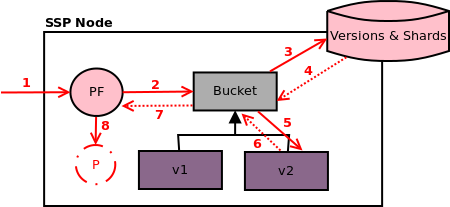
\includegraphics[width=\textwidth]{images/versionsandshards.png}
        \end{column}
    \end{columns}
\end{frame}

\begin{frame}{One API To Rule Them All}
    \begin{itemize}
        \item ``Don't care where it is, just want my data!!!''
        \pause
        \begin{columns}
            \begin{column}[c]{0.6\textwidth}
                    \begin{itemize}
                        \item \href{http://piqi.org}{PIQI}
                        \item Native erlang (+ Protocol Buffers)
                        \item HTTP + JSON
                        \item HTTP + Protocol Buffers
                    \end{itemize}
            \end{column}
            \begin{column}[c]{0.4\textwidth}
                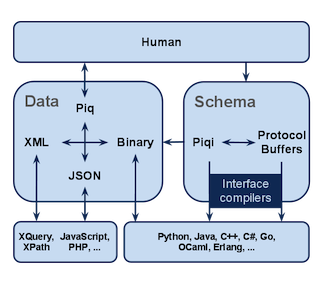
\includegraphics[width=0.8\textwidth]{images/piqi.png}
            \end{column}
        \end{columns}
        \item Protection against code versions!
    \end{itemize}
\end{frame}

\section{Worldwide}

{
\usebackgroundtemplate{
\includegraphics[width=\paperwidth]{images/worldwide.png}}
\begin{frame}{Worlwide}
\end{frame}
}

\subsection{Scaling Datacenters}

\begin{frame}{Masters \& Satellites}
    \begin{columns}
        \begin{column}[c]{0.6\textwidth}
            \begin{itemize}
                \item Master Datacenters
                    \begin{itemize}
                        \item Have persistent storage
                        \item Can own GIDs
                        \item GIDs can be migrated between Master DCs
                    \end{itemize}
                \item Satellite Datacenters
                    \begin{itemize}
                        \item Can't own GIDs
                        \item Don't have persistent storage
                        \item Easy to setup and decommission
                    \end{itemize}
            \end{itemize}
        \end{column}
        \begin{column}[c]{0.4\textwidth}
            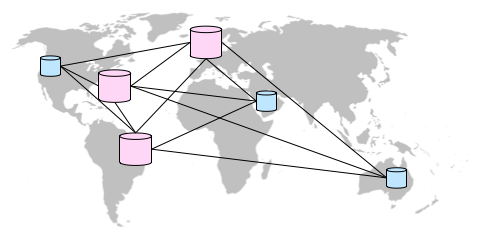
\includegraphics[width=\textwidth]{images/worldmapdc.png}
        \end{column}
    \end{columns}
\end{frame}

\begin{frame}{Working With Multiple Datacenters}
    \begin{columns}
        \begin{column}[c]{0.1\textwidth}
        \end{column}
        \begin{column}[c]{0.8\textwidth}
            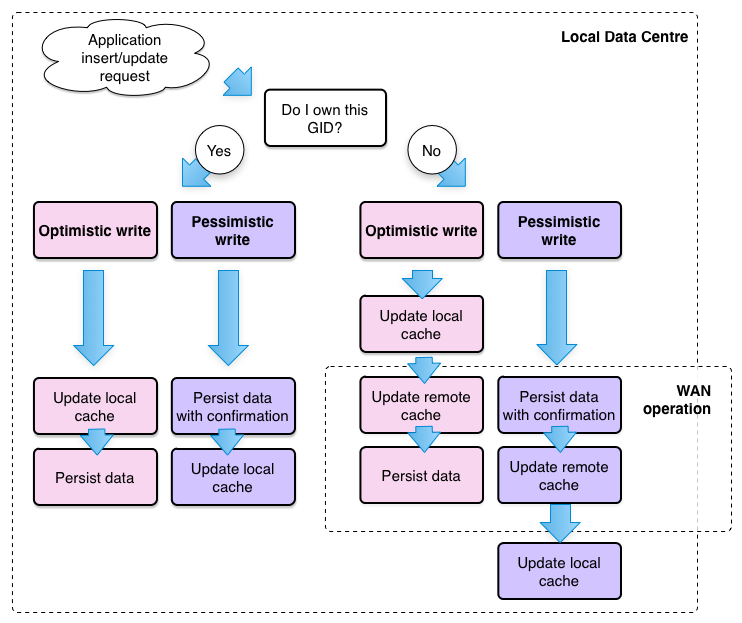
\includegraphics[width=0.8\textwidth]{images/multidcops.png}
        \end{column}
        \begin{column}[c]{0.1\textwidth}
        \end{column}
    \end{columns}
\end{frame}

\begin{frame}{Start With One DC}
    \begin{center}
        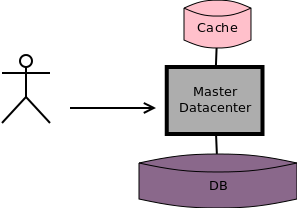
\includegraphics[width=0.4\textwidth]{images/scalingdcs1.png}
    \end{center}
\end{frame}

\begin{frame}{Scale Up A Satellite Where Needed}
    \begin{center}
        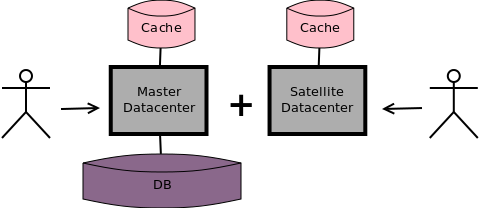
\includegraphics[width=0.7\textwidth]{images/scalingdcs2.png}
    \end{center}
\end{frame}

\begin{frame}{Turn Satellites Into Masters When Ready}
    \begin{center}
        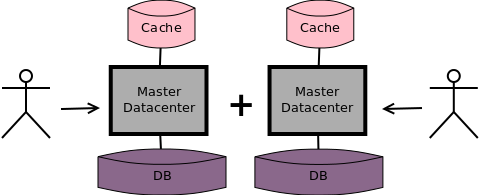
\includegraphics[width=0.7\textwidth]{images/scalingdcs3.png}
    \end{center}
\end{frame}

\subsection{Disaster Scenarios}

{
\usebackgroundtemplate{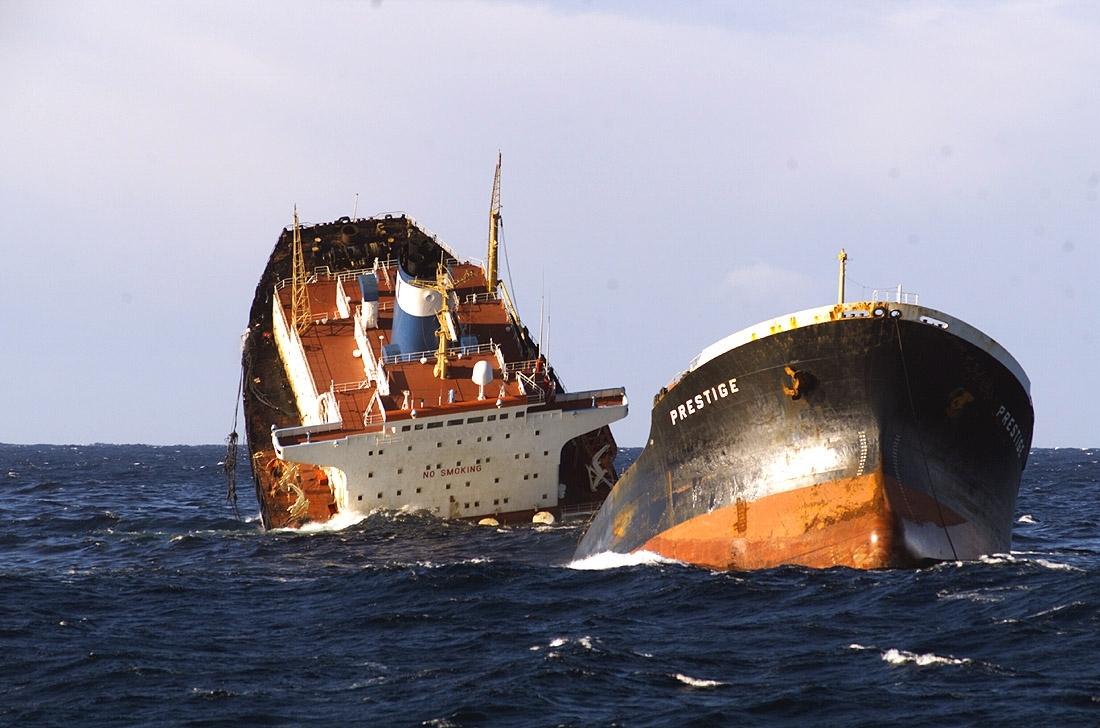
\includegraphics[width=\paperwidth]{images/prestige.png}}
\begin{frame}{Disaster Scenarios}
\end{frame}
}

\begin{frame}{Losing A Satellite Datacenter}
    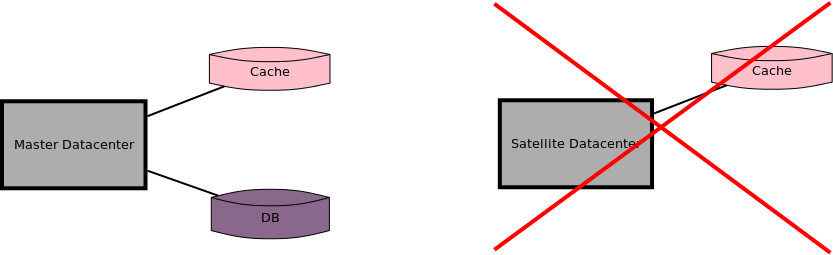
\includegraphics[width=\textwidth]{images/lostsatellitedc.png}
\end{frame}

\begin{frame}{Losing A Master Datacenter}
    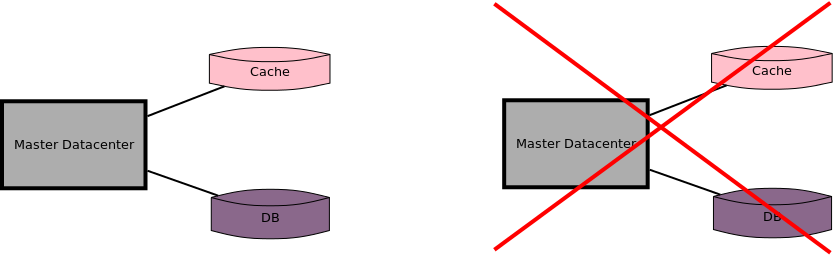
\includegraphics[width=\textwidth]{images/lostmasterdc.png}
\end{frame}

\begin{frame}{Losing A Master Datacenter}
    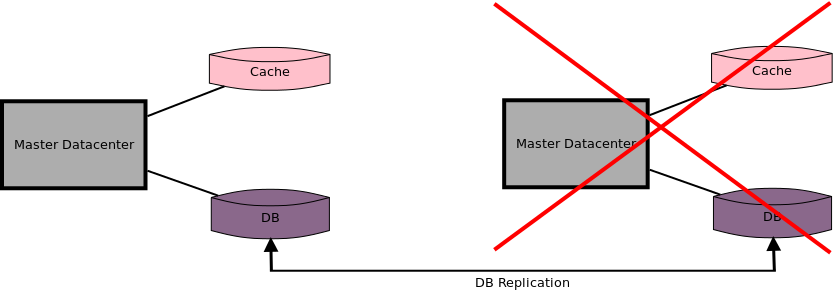
\includegraphics[width=\textwidth]{images/lostmasterdchope.png}
\end{frame}

\section{Lessons Learned}

\subsection{Currents Status}
\begin{frame}{Where We Are}
    \begin{itemize}
        \item Using simple buckets on LIVE in one DC
        \item Added relup support for bucket only updates
        \item Hammering SSP using property based testing
        \item Integrating restricted search capabilities
        \item Testing the WAN protocol for inter DC communication
        \item More buckets to go live in H1 2013
        \item Satellite DCs coming on H2 2013
    \end{itemize}
\end{frame}

\subsection{Contributions}
\begin{frame}{What We've Used}
    \begin{itemize}
        \item Emysql
            \begin{itemize}
                \item (+) multi-database transaction support
                \item (*) multi-timezone support
            \end{itemize}
        \item Eep0018/Jiffy
        \item Estatsd
        \item PropEr
            \begin{itemize}
                \item (*) utf8 generator
            \end{itemize}
        \item Poolboy
        \item Lager
        \item Rebar
            \begin{itemize}
                \item (*) semantic versioning, i.e. [">=1.3.1", "<2.0.0"]
                \item (*) shared dependencies
                \item (*) xref support
            \end{itemize}
        \item Piqi
        \item BashoBench
            \begin{itemize}
                \item (+) Several tests on the same plot support
            \end{itemize}
    \end{itemize}
\end{frame}

\begin{frame}{Questions?}
    \begin{columns}
        \begin{column}[c]{0.5\textwidth}
            
\includegraphics[height=0.9\textheight]{images/holycow.png}
        \end{column}
        \begin{column}[c]{0.5\textwidth}
            
\includegraphics[height=0.8\textheight]{images/questions.png}
        \end{column}
    \end{columns}
\end{frame}

\begin{frame}{That's All Folks!}
    \begin{center}
        \huge{Thanks!}
    \end{center}
\end{frame}

\end{document}

